\documentclass[11pt]{article}
\usepackage[margin=1.0in]{geometry}
\usepackage{ragged2e}
\usepackage{amsmath}    	% Expanded math operations for papers
\usepackage{amssymb}
\usepackage{esvect}    	% Vector notation for mathematics
\usepackage{graphicx}
\usepackage{wrapfig}    	% Format figures more appropriately
\usepackage{hyperref}   	% Enable hyperlink support
\usepackage{fancyhdr}   	% Allow headers and footers customized
\usepackage{titlesec}   	% Allow customization of section headers
\usepackage{wrapfig}    	% So I can wrap figures around my text
\usepackage{enumitem}	% Align things in the itemize environment
\usepackage{xcolor}		% Colored text
\usepackage{subcaption}
\usepackage[font=small,skip=0pt]{caption}

% SI Unit setup
\usepackage{siunitx}
\sisetup{unitsep=\cdot}

% Verilog Programming
\usepackage{listings}

\definecolor{vgreen}{RGB}{104,180,104}
\definecolor{vblue}{RGB}{49,49,255}
\definecolor{vorange}{RGB}{255,143,102}

\lstdefinestyle{verilog}
{
    language=Verilog,
    basicstyle=\small\ttfamily,
    keywordstyle=\color{vblue},
    identifierstyle=\color{black},
    commentstyle=\color{vgreen},
    numbers=left,
    numberstyle=\tiny\color{black},
    numbersep=10pt,
    tabsize=8,
    moredelim=*[s][\colorIndex]{[}{]},
    literate=*{:}{:}1
}

\makeatletter
\newcommand*\@lbracket{[}
\newcommand*\@rbracket{]}
\newcommand*\@colon{:}
\newcommand*\colorIndex{%
    \edef\@temp{\the\lst@token}%
    \ifx\@temp\@lbracket \color{black}%
    \else\ifx\@temp\@rbracket \color{black}%
    \else\ifx\@temp\@colon \color{black}%
    \else \color{vorange}%
    \fi\fi\fi
}
\makeatother

% Set graphics path
\graphicspath{ {figures/} }

% Reformat section headers
\titleformat{\section}{\normalfont\Large\bfseries}{\S\thesection}{1em}{}[{\titlerule[0.8pt]}]
\titleformat{\subsection}{\normalfont\large\bfseries}{\thesection.\Alph{subsection}}{1em}{}
\titleformat{\subsubsection}{\normalfont\normalsize\bfseries}{\thesubsubsection}{1em}{}

% Define page header and footer
\pagestyle{fancy}
\fancyhf{}
\lhead{Alice Seaborn}
\rhead{May 9, 2020}
\lfoot{ECE 482}
\rfoot{Page \thepage}


\begin{document}



%
%%---------------------------------------------------------------------------------------------------| TITLE
%

\begin{Large}\begin{center}
Final Project: Traffic Light Controller
\end{center}\end{Large}


%
%%---------------------------------------------------------------------------------------------------| PROMPT
%

\section{Project Statement}

Use system verilog to develop a controller unit for a simple two street intersection complete with corresponding lights and traffic sensors. Given that the configuration of the lights is finite, a state-machine approach is logical to describe the intersection's behavior. The lights will remain in their current state until the sensors on the opposing street trigger a change in traffic flow. In such a case, a transient state occurs which slows the current traffic prior to introducing opposing traffic.


%
%%---------------------------------------------------------------------------------------------------| DIAGRAM
%

\section{State Diagram}

Given the sensory inputs and the procedural flow of some states logically into other states (e.g. green through red cycle) the following state truth table can be derived:

\begin{figure}[h!]
\centering
\begin{tabular}{|c|c|c|}
	\hline
	\textbf{Present state}	& \textbf{Next state}	& \textbf{Output}	\\
	\hline
	state0	&	(0,0) $\rightarrow$ state1	&	$green1 = 1$, $red2 = 1$	\\
			&	(0,1) $\rightarrow$ state2	&	N-S street open			\\
			&	(1,0) $\rightarrow$ state0	&							\\
			&	(1,1) $\rightarrow$ state1	&							\\
	\hline
	state1	&	state2						&	$green1 = 1$, $red2 = 1$	\\
	\hline
	state2 	&	state3						&	$green1 = 1$, $red2 = 1$	\\
	\hline
	state3	&	state4						&	$yellow1 = 1$, $red2 = 1$\\
			&								&	Unprotected left			\\
	\hline	
	state4	&	(0,0) $\rightarrow$ state5	& 	$red1 = 1$, $green2 = 1$	\\
			&	(0,1) $\rightarrow$ state4	&							\\
			&	(1,0) $\rightarrow$ state6	&							\\
			&	(1,1) $\rightarrow$ state4	&							\\
	\hline
	state5	&	state6						&	$red1 = 1$, $green2 = 1$	\\
	\hline
	state6	&	state7						&	$red1 = 1$, $green2 = 1$	\\
	\hline
	state7	&	state0						&	$red1 = 1$, $yellow2 = 1$\\
	\hline
\end{tabular}
\vspace{0.2cm}
\caption{State truth table.}
\end{figure}

\noindent From this truth table, a more detailed flow diagram has been produced below.

\begin{figure}[h!]
	\centering
	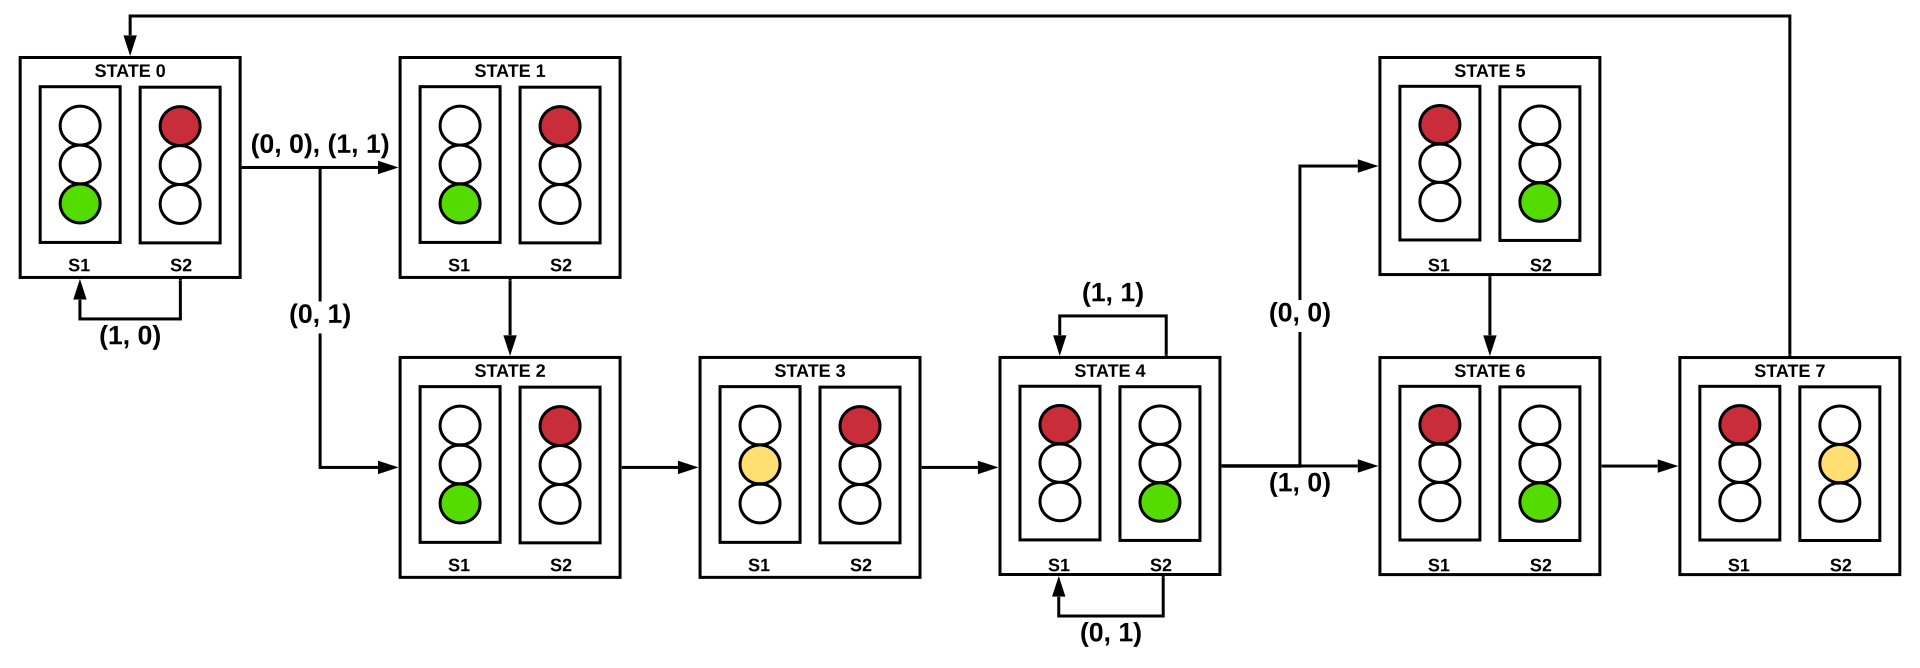
\includegraphics[width=0.85\textwidth]{Flow-Diagram.png}
	\caption{Traffic Light Controller flow diagram.}
\end{figure}


%
%%---------------------------------------------------------------------------------------------------| APPROACH
%

\section{Solution Approach}

In order to describe the behavior of the controller, a local variable was used to define the current state. This variable is a customized enumeration that lists the possible states for the controller unit.

\begin{lstlisting}[style=verilog]
typedef enum {state0, state1, state2, state3, state4,
	state5, state6, state7} state_t;

// Define state enumeration variables
state_t state, next_state;
\end{lstlisting}

System Verilog allows for switch case statements to be applied to enumeration variables. Ergo, the remainder of the solution can be solved in a single large switch case against the current state. To prevent against confusing the system, the $next_state$ variable is used to delay updating the current state until the next switch case iteration like so:

\begin{lstlisting}[style=verilog]
always_ff @(posedge clk, posedge reset)
	begin
		if(reset)
			state = state0;
		else
			state = next_state;
	end
\end{lstlisting}

From there, the switch case explicitly defines the logic described by both the flow diagram as well as the state truth table. When simulating the controller, the clock must be modified to slow the system. Rather than adjusting the time signature, a clock divider can be implemented where \textit{T} is a finite local parameter\footnote{Similar to a \textit{\#define} statement in C-languages.}

\begin{lstlisting}[style=verilog]
// Divide clock manually
  always
    begin
      clk = 1;
      #(T/2);
      clk = 0;
      #(T/2);
    end
\end{lstlisting}

Then the testbench can iterate between signal configurations by explicitly changing the sensory input and waiting for the states to change, again as a function of the local parameter \textit{T}:

\begin{lstlisting}[style=verilog]
sen1 = 0;
sen2 = 0;
#(T*5);

sen1 = 1;
sen2 = 0;
#(T*5);

sen1 = 0;
sen2 = 1;
#(T*5);
...
\end{lstlisting}

The code is then loaded into EDA Playground in an environment which can be accessed through the link included below. The Mentor Questa simulator is used and the wave output is included in the figure below.

\begin{center}
\url{https://www.edaplayground.com/x/6NwQ}
\end{center}

\begin{figure}[h!]
	\includegraphics[width=\textwidth]{wave.png}
	\caption{EPWave output from TLC simulation.}
\end{figure}



\end{document}

